\documentclass[12pt]{article}
\usepackage[utf8]{inputenc}
\usepackage{float}
\usepackage{amsmath}
\usepackage{tikz}

\usepackage[hmargin=3cm,vmargin=6.0cm]{geometry}
%\topmargin=0cm
\topmargin=-2cm
\addtolength{\textheight}{6.5cm}
\addtolength{\textwidth}{2.0cm}
%\setlength{\leftmargin}{-5cm}
\setlength{\oddsidemargin}{0.0cm}
\setlength{\evensidemargin}{0.0cm}

%misc libraries goes here



\begin{document}

\section*{Student Information } 
%Write your full name and id number between the colon and newline
%Put one empty space character after colon and before newline
Full Name :  Berkay Bartuğ Çetin\\
Id Number : 2309839\\

% Write your answers below the section tags
\section*{Answer 1}
a)


\begin{tabular}{ll|l|ll} 
\cline{3-3}
                              &                      & \{1,2,3\}            &                       &                               \\ 
\hline
\multicolumn{1}{|l|}{\{1,2\}} &                      & \{1,3\}              & \multicolumn{1}{l|}{} & \multicolumn{1}{l|}{\{2,3\}}  \\ 
\hline
\multicolumn{1}{|l|}{\{1\}}   &                      & \{3\}                & \multicolumn{1}{l|}{} & \multicolumn{1}{l|}{\{2\}}    \\ 
\hline
                              &                      & \{\}                 &                       &                               \\ 
\cline{3-3}
                              & \multicolumn{1}{l}{} & \multicolumn{1}{l}{} &                       &                               \\
                              & \multicolumn{1}{l}{} & \multicolumn{1}{l}{} &                       &                               \\
                              & \multicolumn{1}{l}{} & \multicolumn{1}{l}{} &                       &                              
\end{tabular}
\\
b) Every element pairs have both upper and greatest lower bound, so it is a lattice. \\
c) Maximal element $\{a,b,c\}$ whic is above all adjacent nodes. \\
d) Minimal element $\{\}$ whis is under every other node.\\
e) All other nodes are the subset of $\{ a,b,c \}$ , therefore $\{ a,b,c \}$ is the greatest element. \\
f) There is no node which is a subset of $\{\}$, hence $\{\}$ is the least element. \\
g) $\{1,3\}$ is least upper bound of $\{1\}$ and $\{3\}$. \\

\section*{Answer 2}
a) $degree(a) = 2, degree(b) = 4, degree(c) = 2, degree(d) = 3 ,degree(e) = 3$. When we sum them up, result is 14.\\
b) It equals to the sum of degrees of all nodes which is 14. \\
c) Number of edges is 7, so there are $7*2=14$ non-zero entries in the incidence matrix representation. \\
d) Yes it does. \\
\begin{figure}[H]
	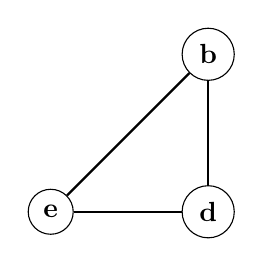
\begin{tikzpicture}
	
	\node[shape=circle,draw=black] (b) at (2, 2)     {\textbf{b}};
	\node[shape=circle,draw=black] (d) at (2, 0)     {\textbf{d}};
	\node[shape=circle,draw=black] (e) at (0, 0)     {\textbf{e}};
	
	\path[-, thick] (b) edge (e);
	\path[-, thick] (b) edge (d);
	\path[-, thick] (d) edge (e);
	
	\end{tikzpicture} 

\end{figure}
\newpage
e) No, G is not a bipartite. Because we end up with neighbors with same color.\\
\begin{figure}[H]
	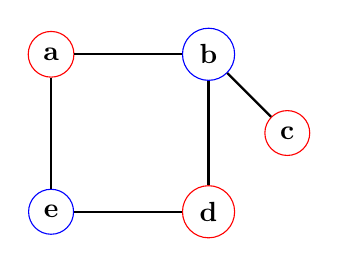
\begin{tikzpicture}
	
	\node[shape=circle,draw=red] (a) at (0, 2)     {\textbf{a}};
	\node[shape=circle,draw=blue] (b) at (2, 2)     {\textbf{b}};	
	\node[shape=circle,draw=red] (c) at (3, 1)     {\textbf{c}};	
	\node[shape=circle,draw=red] (d) at (2, 0)     {\textbf{d}};
	\node[shape=circle,draw=blue] (e) at (0, 0)     {\textbf{e}};
	
	\path[-, thick] (a) edge (b);
	\path[-, thick] (a) edge (e);
	\path[-, thick] (b) edge (d);
	\path[-, thick] (e) edge (d);
	\path[-, thick] (b) edge (c);
	
	\end{tikzpicture} 

\end{figure}

f) $2^7$ because every edge (7edges) might have 2 different directions. \\
g) 5, the path is a-b-c-d-e.\\
h) 1 because all nodes are connected to each other. \\
i) Yes. For example $\{e, a, b, e, d, c, b, d\}$ is a Euler Circuit. \\
j) No, because there is more than 2 vertices with odd degree. \\
k) Yes, there is a Hamilton Circuit. \{a,b,c,d,e,a\}\\
l) Yes, there is a Hamilton Path. \{a,b,c,d,e\}\\

\section*{Answer 3}
Yes they are isomorphic. \\
They have the same number of vertices.\\
They have the same number of edges.\\
They have the same degree sequence.\\
Relation between nodes of two graphs is;\\
$a' = f(a), b' = f(e), c' = f(b), d' = f(g)$\\
$e' = f(c), f' = f(h) ,g' = f(d), h' = f(f)$\\

\newpage
\section*{Answer 4}
Step1) Box out a and $D(a)=0$, traverse the neighbors of a; $D(b)=4, D(e)=5, D(h)=4$. \\
Step2) Box out b which has the smallest distance $D(b)=3$; D(e) stayed the same,\\ $D(f)=10, D(c)=5$. \\
Step3) Box out h which has the smallest distance $D(h)=4$; $D(i)=6, D(f) is changed to 9$. \\
Step4) Box out e which has the smallest distance $D(e)=5$; D(f) stayed the same. \\
Step5) Box out c which has the smallest distance $D(c)=5$; D(f) changed to 7$, D(d)=8, D(g)=11$. \\
Step6) Box out i which has the smallest distance $D(i)=6$; D(f) stayed the same, $D(j)=12$ \\
Step7) Box out f which has the smallest distance $D(f)=7$; D(g) stayed the same, \\D(j) changed to 10. \\
Step8) Box out d which has the smallest distance $D(d)=8$; D(g) stayed the same, $D(k)=10$. \\
Step9) Box out j which has the smallest distance $D(j)=10$; D(g) stayed the same, \\ D(k) stayed the same. \\
Step10) Box out k which has the smallest distance $D(k)=10$; D(g) stayed the same. \\
Step11) Box out g which has the smallest distance $D(g)=11$; No change.
Finally resulting distances at the nodes are: \\
$D(a) = 0$, \\
$D(b) = 3$, \\
$D(c) = 5$, \\
$D(d) = 8$, \\
$D(e) = 5$, \\
$D(f) = 7$,\\
$D(g) = 11$, \\
$D(h) = 4$, \\
$D(i) = 6$, \\
$D(j) = 10$, \\
$D(k) = 10$. \\

\newpage
\section*{Answer 5}
a) Visited = \{a,b,d,c,f,e\} \\
$E(a,b) \rightarrow E(a,d) \rightarrow E(b,c) \rightarrow E(c,f) \rightarrow E(f,e)$ \\
\\ b) 
\begin{figure}[H]
	\centering
	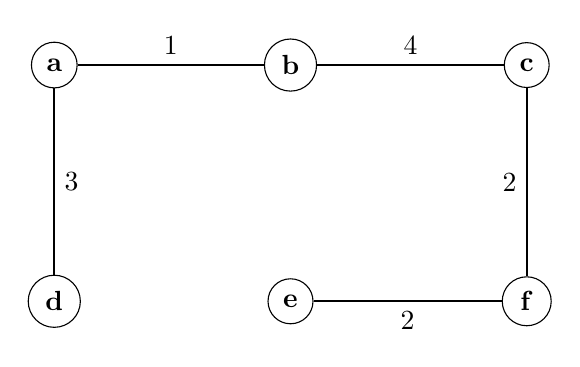
\begin{tikzpicture}
	
	\node[shape=circle,draw=black] (a) at (0, 3)     {\textbf{a}};
	\node[shape=circle,draw=black] (b) at (3, 3)     {\textbf{b}};
	\node[shape=circle,draw=black] (c) at (6, 3)     {\textbf{c}};
	\node[shape=circle,draw=black] (d) at (0, 0)     {\textbf{d}};
	\node[shape=circle,draw=black] (e) at (3, 0)     {\textbf{e}};
	\node[shape=circle,draw=black] (f) at (6, 0)     {\textbf{f}};
	
	\path[-, thick] (a) edge node[above]{1} (b);
	\path[-, thick] (b) edge node[above]{4} (c);
	\path[-, thick] (a) edge node[right]{3} (d);
	\path[-, thick] (c) edge node[left]{2} (f);
	\path[-, thick] (e) edge node[below]{2} (f);
	
	\end{tikzpicture} 
\end{figure}



c) Yes, choosen minimum spanning tree is unique because edge weights are distincnt and unique for it.

\section*{Answer 6}
a) There are 13 vertices, 12 edges and $Height(T)=4$ \\
b) w, s, m, t, q, x, n, y, u, z, v, r, p. \\
c) s, w, q, m, t, p, x, u, n, y, r, v, z. \\
d) p, q, s, w, t, m, r, u, x, y, n, v, z. \\
e) No it is not because every node other than leaf nodes must have 2 children but node(y) has only 1 child.\\

\end{document}